\documentclass[a4paper,12pt]{report}
\usepackage{graphicx}
\graphicspath{{picaa/}}
\usepackage{listings}
\usepackage{amsmath}
\usepackage[T2A]{fontenc}
\usepackage[utf8]{inputenc}
\usepackage[english,russian]{babel}
\usepackage{pgfplots} 
\usepackage{indentfirst}
\parindent=1cm

\usepackage{longtable}
\usepackage{geometry}
\geometry{left=2cm}
\geometry{right=1.5cm}
\geometry{top=1cm}
\geometry{bottom=2cm}
\lstset{language = C++,
	keywordstyle = \color{orange},
	commentstyle = \color{red},
	columns = fullflexible
}

\begin{document}

    \begin{titlepage}

        \begin{center}
            \large
            \textbf{Государственное образовательное учреждение высшего профессионального образования\\
            “Московский государственный технический университет имени Н.Э.Баумана”\\}
            
\includegraphics{bmstu-logo.png}
			\vspace{1cm}
            
            \textsc{Дисциплина: Анализ алгоритмов}
            \vspace{0.5cm}
                
            \textsc{Лабораторная работа №7}
            \vspace{1cm}
            
            {\LARGE \textbf{Поиск подстроки в строке}}
            \vspace{3cm}
                    
            \begin{flushright}
            	Студент группы ИУ7-55Б,\\   
            	Руднев К. К.,\\
            	\vspace{0.5cm}
            	Преподаватель,\\
            	Волкова Л. Л.,\\
            	Строганов Ю. В.
            	
            \end{flushright}
            \vfill
            
            2019 г.
            
            \end{center}

    \end{titlepage}

	\setcounter{page}{2}
	\tableofcontents
    \chapter*{Введение}

        	Цель работы: изучение алгоритмов поиска подстроки в строке.
        	
        	Задачи данной лабораторной работы:
        	\begin{enumerate}
        		\item изучить алгоритмы Бойера-Мура и Кнута-Морриса-Пратта;
        		\item реализовать эти алгоритмы;
        		\item провести тестирование ПО.
        	\end{enumerate}
        \label{sec:intro}

    \newpage

    \chapter{Аналитическая часть}
        \label{sec:analitic_part}
        
        	В рамках раздела будут рассмотрены алгоритмы поиска подстроки в строке.
		
	\section{Общие сведения об алгоритмах поиска подстроки в строке}
        
			Поиск подстроки в строке — одна из простейших задач поиска информации. 
			Применяется в виде встроенной функции в текстовых редакторах, СУБД, поисковых машинах, языках программирования, программы определения плагиата осуществляют онлайн-проверку, используя алгоритмы поиска подстроки среди большого количества документов, хранящихся в собственной базе\cite{1}.
			
			На сегодняшний день существует огромное разнообразие алгоритмов поиска подстроки. 
			Программисту приходится выбирать подходящий в зависимости от таких факторов: длина строки, в которой происходит поиск, необходимость оптимизации, размер алфавита, возможность проиндексировать текст, требуется ли одновременный поиск нескольких строк. 
			
			В данной лабораторной работе будут рассмотремы два алгоритма сравнения с образцом, алгоритм Кнута-Морриса-Пратта и алгоритм Бойера-Мура.

	\subsection{Стандартный алгоритм}

		Стандартный алгоритм начинает со сравнения первого символа текста с первым символом подстроки. 
		Если они совпадают, то происходит переход ко второму символу текста и подстроки. 
		При совпадении сравниваются следующие символы. 
		Так продолжается до тех пор, пока не окажется, что подстрока целиком совпала с отрезком текста, или пока не встретятся несовпадающие символы. 
		В первом случае задача решена, во втором мы сдвигаем указатель текущего положения в тексте на один символ и заново начинаем сравнение с подстрокой\cite{2}.
		
	\subsection{Алгоритм Бойера-Мура}

		Алгоритм Бойера-Мура осуществляет сравнение с образцом справа налево, а не слева направо. 
		Исследуя искомый образец, можно осуществлять более эффективные прыжки в тексте при обнаружении несовпадения. 
		В этом алгоритме кроме таблицы суффиксов применяется таблица стоп-символов. 
		Она заполняется для каждого сивола в алфавите. 
		Для каждогостречающегося в подстроке символа таблица заполняется по принципу максимальной позиции символа в строке, за исключением последнего символа. 
		При определении сдвига при очередном несовпадении строк, выбирается максимальное значение из таблицы суффиксов и стоп-символов\cite{2}.
		
	\subsection{Алгоритм Кнута-Морриса-Пратта}	
		
		Алгоритм Кнута-Морриса-Пратта основан на принципе конечного автомата, однако он использует более простой метод обработки неподходящих символов. 
		В этом алгоритме состояния помечаются символами, совпадение с которыми должно в данный момент произойти. 
		Из каждого состояния имеется два перехода: один соответствует успешному сравнению, другой - несовпадению. 
		Успешное сравнение переводит нас в следующий узел автомата, а в случае несовпадения мы попадаем в предыдущий узел, отвечающий образцу.
		 
		В программной реализации этого алгоритма применяется массив сдвигов, который создается для каждой подстроки, которая ищется в тексте. 
		Для каждого символа из подстроки рассчитывается значение, равное максимальной длине совпадающего префикса и суффикса отсительно конкретного элемента подстроки. 
		Создание этого массива позволяет при несовпадении строки сдвигать ее на расстояние, большее, чем 1 (в отличие от стандартного алгоритма).
		
	\section{Вывод}

		В данном разделе были рассмотрены основные алгоритмы поиска подстроки в строке.
	
    \newpage

    \chapter{Конструкторская часть}
        \label{sec:construct_part}
        
			В данном разделе будут рассмотрена пошаговая работа алгоритмов.

	\section{Разработка алгоритмов}
		
		В таблице \ref{table:kmp} и \ref{table:bm} будет рассмотрена пошаговая работа алгоритмов Кнута-Морриса-Пратта и Бойера-Мура на значениях строки s и подстроки sub.  
		\vspace{0.5cm}
		\newline
		string s = "ababacabaa"; 
		\newline 
		string sub = "abaa";  
		
	 \subsection{Алгоритм Кнута-Морриса-Пратта}
 
 		Для алгоритма Кнута-Морриса-Пратта вычисленный массив префиксов для заданой  подстроки sub имеет значение:
 		prefix = [0, 0, 1, 1]
 		
 		Таблица \ref{table:kmp} отображает пошаговую работу алгоритма Кнута-Морриса-Пратта при данном массиве префиксов.
 			
 			\begin{longtable}{| c | c | c | c | c | c | c | c | c | c | }
				\caption{Пошаговая работа алгоритма Кнута-Морриса-Пратта}
				\label{table:kmp}\\
 				\hline
 				a&b&a&b&a&c&a&b&a&a \\
 				\hline
 				\hline
 				a&b&a&\textcolor{red}{a}&&&&&&\\
 				\hline
 				&&a&b&a&\textcolor{red}{a}&&&&\\
 				\hline
 				&&&&a&\textcolor{red}{b}&a&a&&\\
 				\hline
 				&&&&&\textcolor{red}{a}&b&a&a&\\
 				\hline
 				&&&&&&a&b&a&\textcolor{green}{a}\\
 				\hline
 			\end{longtable}
	
	\subsection{Алгоритм Бойера-Мура}
	
		Для алгоритма Бойера-Мура вычисленный массив суффиксов для заданой  подстроки sub имеет значение:
		suffix = [2, 5, 5, 6].
		Переходы алфавита для подстроки sub:
		letters = ['a' = 0, 'b' = 2].
		Если буквы нет в letters, будет считаться, что переход равен длиние sub.
			
			\begin{longtable}{| c | c | c | c | c | c | c | c | c | c | }
				\caption{Пошаговая работа алгоритма Бойера-Мура}
				\label{table:bm}\\
				\hline
				a&b&a&b&a&c&a&b&a&a \\
				\hline
				\hline
				a&b&a&\textcolor{red}{a}&&&&&&\\
				\hline
				&&a&b&a&\textcolor{red}{a}&&&&\\
				\hline
				&&&&&&\textcolor{green}{a}&b&a&a\\
				\hline
			\end{longtable}
	
	\section{Вывод}

		В данном разделе была разобрана работа алгоритмов на конкретных входных данных.

    \newpage

    \chapter{Технологическая часть}
    
        \label{sec:tecnologic_part}
			В рамках раздела будут описаны инструментарии разработки, выбор среды, требования к ПО. 
			Также будут предоставлены листинги конкретных реализаций алгоритмов.
			
			Замеры времени были произведены на: Intel(R) Core(TM) i7-8565U, 4 ядра, 8 логических процессоров.
	
	\section{Средства реализации}
			
			Для реализации алгоритмов использовался язык программирования C++ 17 и среда разработки QtCreator Community Edition 5.5. 
        	У данного языка имеются удобные библиотеки для написания мультипоточных приложений, чего будет достаточно для реализации текущей лабораторной работы, а среда разработки имеет бесплатную коммьюнити версию и подходящий компилятор.
        	
        	Замер времени реализован с помощью функции clock() из библиотеки time.h.
        	Измеряется время исполнения кода чистого алгоритма (без учета времени на создание потоков, очередей, генерацию данных и т.п.).

	\section{Требования к программному обеспечению}

			На вход программа должна получать строку и подстроку, которую необходимо найти. 
			
			На выход программа должна вернуть индекс начала совпадения или -1, если подстрока не содержится в данной строке. 

	\section{Листинг кода}
	
        	На листингах \ref{list:std}-\ref{list:kmp} представлена реализация конвейерной обработки данных.
	        На листинге \ref{list:std} представлен код стандартного алгоритма поиска подстроки в строке.
	        На листинге \ref{list:bm} представлен код алгоритма Бойера-Мура.
	        На листинге \ref{list:kmp} представлен код алгоритма Кнута-Морриса-Пратта.
	        
	        \begin{lstlisting}[frame = single, breaklines, label = list:std, caption = Стандартный алгоритм]
	int find(string text, string substr)
	{
	    for (int i = 0; i < text.length(); ++i)
	    {
	        int j = 0;
	        for (j = 0; j < substr.length(); ++j)
	        {
 	            if(text[i+j] != substr[j])
	                break;
	        }
	        if (j == substr.length())
	            return i;
	    }
	    return -1;
	}
	        \end{lstlisting}
	        	
	        \begin{lstlisting}[frame = single, breaklines, label = list:bm, caption = Алгоритм Бойера-Мура]
	bool isPrefix(const std::string &substr, const int &p)
	{
	    int j = 0;
	    for (int i = p; i < substr.length(); ++i)
	    {
	        if (substr[i] != substr[j])
	            return false;
	        j++;
	    }
	    return true;
	}
	
	int suffixLength(const std::string &substr, const int &p)
	{
	    int len = 0;
	    int i = p, j = substr.length() - 1;
	    while (i >= 0 && substr[i] == substr[j])
	    {
	        len++;
	        i--;
	        j--;
	    }
	    return len;
	}
	
	std::vector<int> getSuffix(const std::string &substr)
	{
	    int n = substr.length();
	    std::vector<int> table(n);
	    int lastPrefixPosition = n;
	
	    for (int i = n - 1; i >= 0; --i)
	    {
	        if (isPrefix(substr, i + 1))
	        lastPrefixPosition = i + 1;
	        table[n - 1 - i] = lastPrefixPosition - i + n - 1;
	    }
	
	    for (int i = 0; i < n - 1; i++)
	    {
	        int slen = suffixLength(substr, i);
	        table[slen] = n - 1 - i + slen;
	    }
	
	    return table;
	}
	
	int searchBM(const std::string &text, const std::string &substr)
	{
	    std::unordered_map<char, int> stopTable;
	    int m = substr.length();
	    int n = text.length();
	    std::vector<int> suffix = getSuffix(substr);
	    for (int i = 0; i < m; ++i)
	    {
	        stopTable[substr[i]] = m - 1 - i;
	    }
	
	    for (int i = m - 1; i < n;)
	    {
	        int j = m - 1;
	
	        while (substr[j] == text[i])
	        {
	            if (j == 0)
	                return i;
	            i--;
	            j--;
	        }
	        auto stop_symbol = stopTable.find(text[i]);
	        int stopAdd = stop_symbol != stopTable.end() ? stop_symbol->second : m;
	        i += std::max(suffix[m - j - 1], stopAdd);
	    }
	    return -1;
	}
	        \end{lstlisting}
	
	        \begin{lstlisting}[frame = single, breaklines, label = list:kmp, caption = Алгоритм Кнута-Морриса-Пратта]
	string::size_type KMP(const string& S, const string& pattern)
	{
	    vector<int> pf (pattern.length());
	
	    pf[0] = 0;
	    for (int k = 0, i = 1; i < pattern.length(); ++i)
	    {
	        while ((k > 0) && (pattern[i] != pattern[k]))
	        k = pf[k-1];
	
	        if (pattern[i] == pattern[k])
	            k++;
	
	        pf[i] = k;
	    }
	
	    for (int k = 0, i = 0; i < S.length(); ++i)
	    {
	        while ((k > 0) && (pattern[k] != S[i]))
	            k = pf[k-1];
	
	        if (pattern[k] == S[i])
	            k++;
	
	        if (k == pattern.length())
	            return (i - pattern.length() + 1);
	    }
	    return -1;
	}
	        \end{lstlisting}
	      
	\section{Вывод}
	
		В рамках раздела были предъявлены требования к программному обеспечению. 
		На основании их были разработаны и представлены конкретные реализации стандартного алгоритма, алгоритма Кнута-Морриса-Пратта и алгоритма Бойера-Мура для нахождения подстроки в данной строке.      
	        
    \newpage

    \chapter{Экспериментальная часть}
        \label{sec:experimental_part}

			В этом разделе будет проведен сравнительный анализ алгоритмов поиска подстроки в строке. 
			На рисунках \ref{ris:test1} - \ref{ris:test3} приведены результаты теств программы.

	\section{Примеры работы}

		\begin{figure}[h!]
			\center{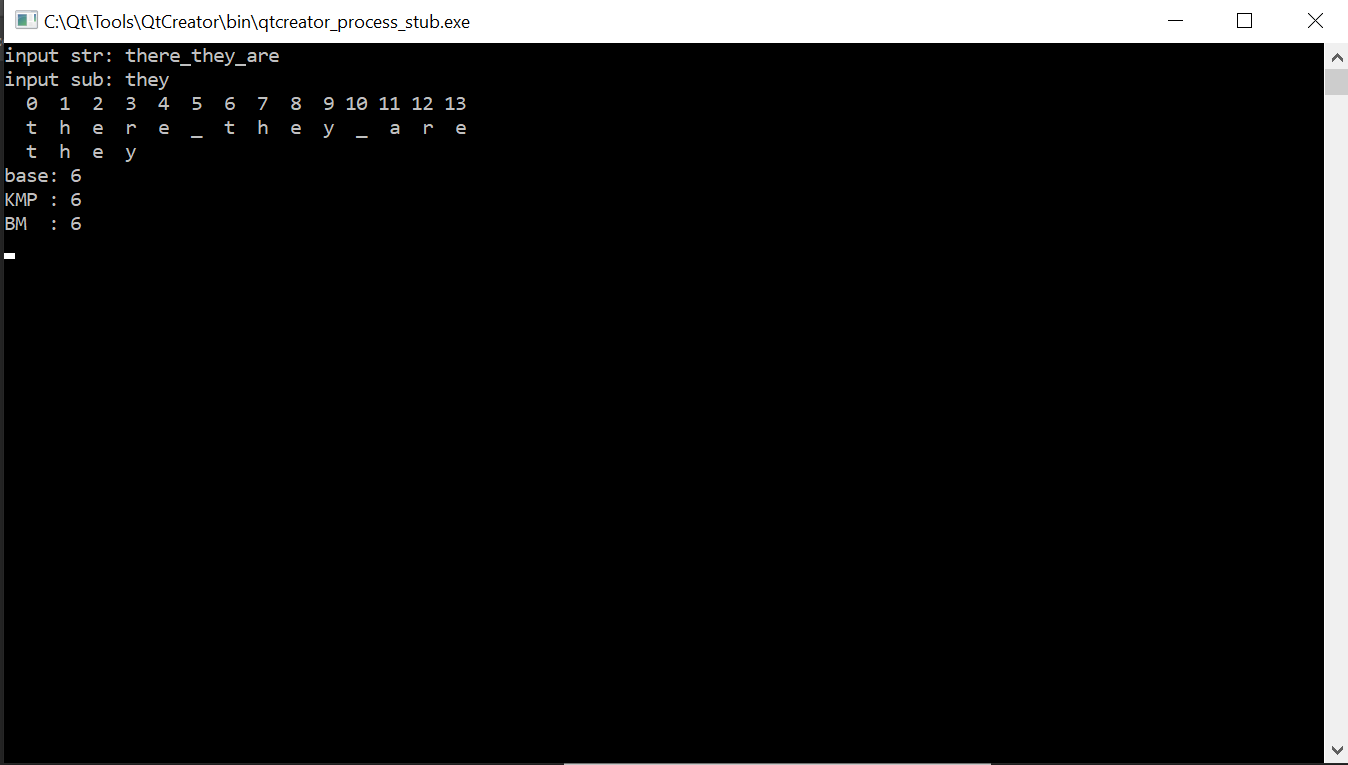
\includegraphics[width=0.8\linewidth]{find_p1.png}}
			\caption{Пример работы 1}
			\label{ris:test1}
		\end{figure}
	
		\begin{figure}[h!]
			\center{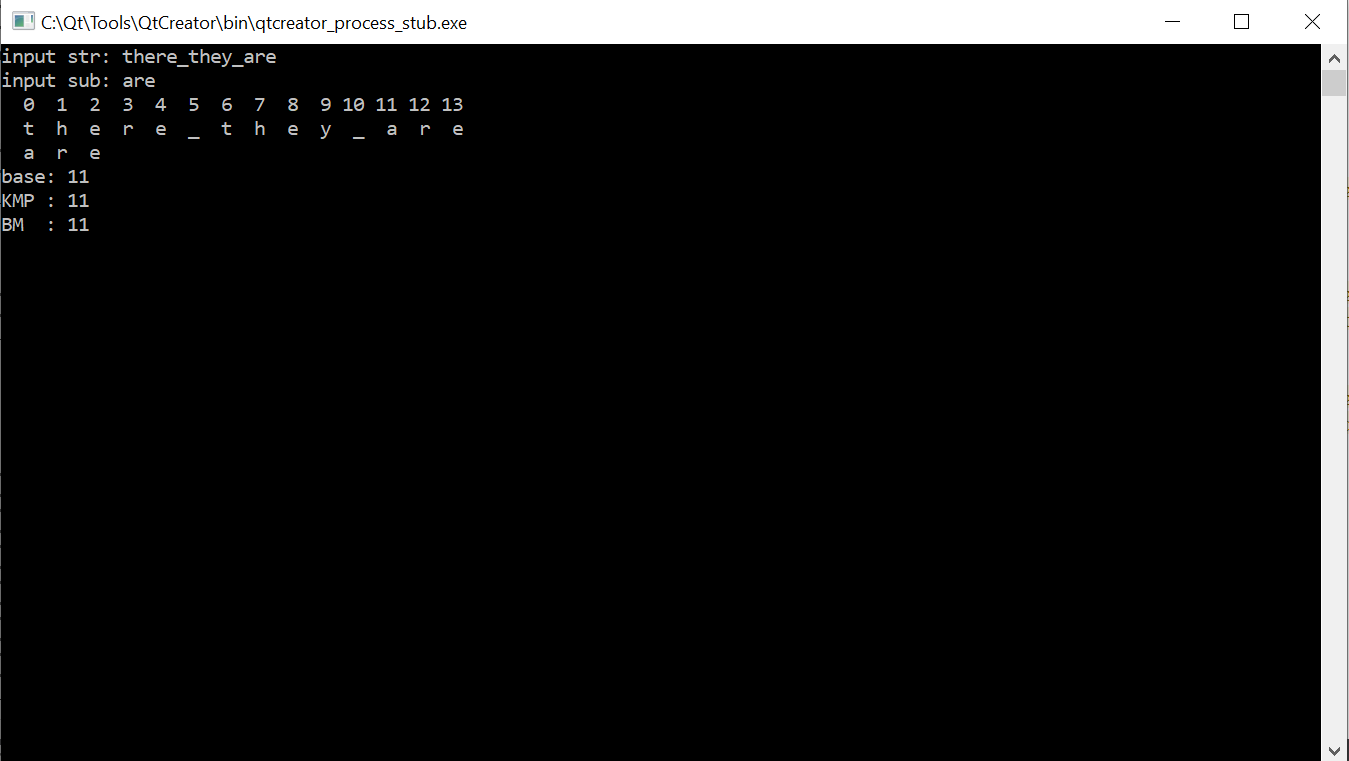
\includegraphics[width=0.8\linewidth]{find_p2.png}}
			\caption{Пример работы 2}
			\label{ris:test2}
		\end{figure}
	
		\newpage
	
		\begin{figure}[h!]
			\center{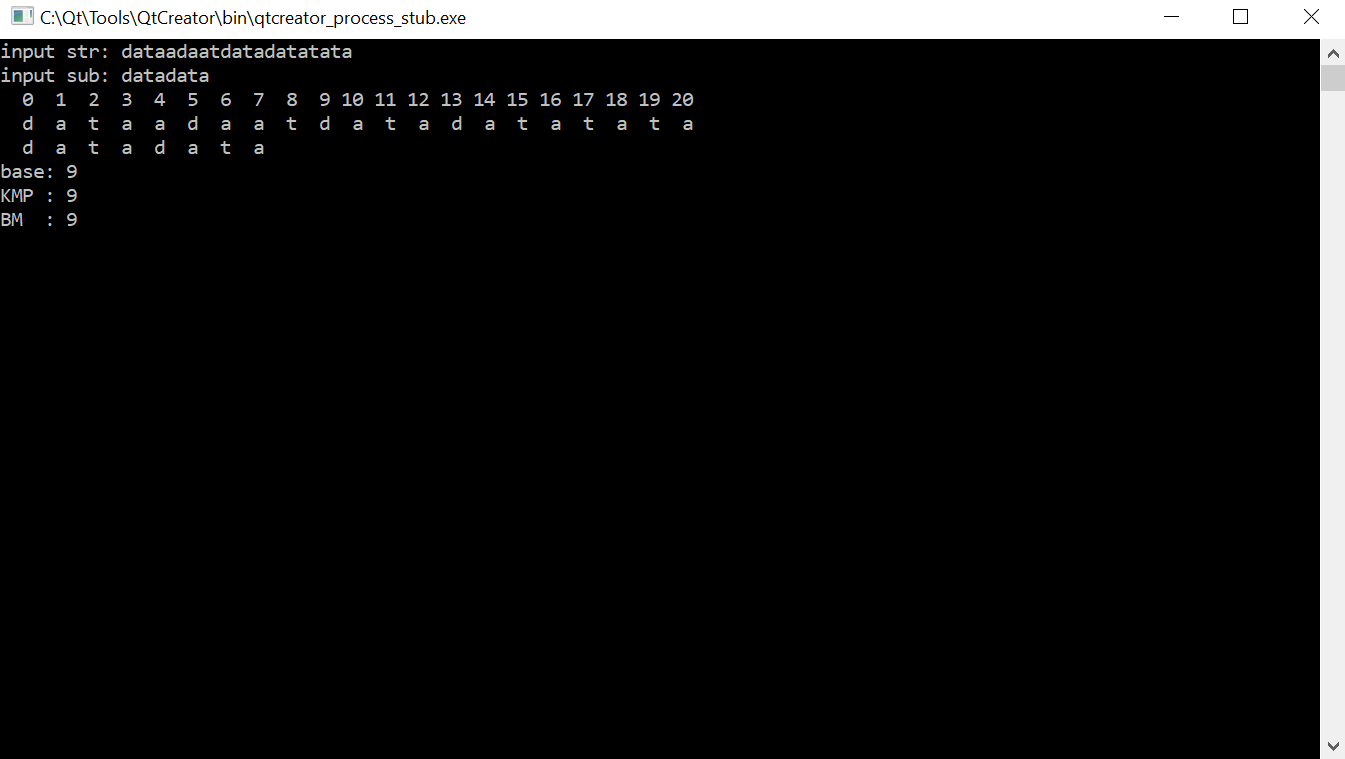
\includegraphics[width=0.8\linewidth]{find_p3.png}}
			\caption{Пример работы 3}
			\label{ris:test3}
		\end{figure}
        
    \section{Постановка эксперимента} 

		Были проведены временные эксперименты для строк  от 1 000 до 100 000 элементов с шагом 1000. 
		Для каждого замера взят средний результат из 100 замеров.  
		Замеры проведены для трех случаев: длина подстроки 4 символа, длина подстроки 12 символов и длина подстроки 20 символов. 
		Результаты экспериментов представлены на рисунках \ref{graph:len4}-\ref{graph:len20}.

		\begin{figure}[h!]
			\begin{tikzpicture}
			\begin{axis}[
			height = 300,
			width = 500,
			axis lines = left,
			xlabel = {Длина},
			ylabel = {Время (тики)},
			legend pos=north west,
			ymajorgrids=true
			]
			
			\addplot[color=blue] table[x index=0, y index= 1] {std.txt}; 
			\addlegendentry{Стандартный}
			
			\addplot[color=orange] table[x index=0, y index= 1] {bm.txt}; 
			\addlegendentry{BM}
			
			\addplot[color=red] table[x index=0, y index= 1] {kmp.txt}; 
			\addlegendentry{KMP}
			
			\end{axis}
			\end{tikzpicture}
			\caption{Сравнение времени работы алгоритмов при фиксированной длине подстроки, равной 4}
			\label{graph:len4}
		\end{figure}   
	
		\newpage
	
		\begin{figure}[h!]
			\begin{tikzpicture}
			\begin{axis}[
			height = 300,
			width = 500,
			axis lines = left,
			xlabel = {Длина},
			ylabel = {Время (тики)},
			legend pos=north west,
			ymajorgrids=true
			]
			
			\addplot[color=blue] table[x index=0, y index= 1] {std12.txt}; 
			\addlegendentry{Стандартный}
			
			\addplot[color=orange] table[x index=0, y index= 1] {bm12.txt}; 
			\addlegendentry{BM}
			
			\addplot[color=red] table[x index=0, y index= 1] {kmp12.txt}; 
			\addlegendentry{KMP}
			
			\end{axis}
			\end{tikzpicture}
			\caption{Сравнение времени работы алгоритмов при фиксированной длине подстроки, равной 12}
			\label{graph:len12}
		\end{figure} 
	
		\begin{figure}[h!]
			\begin{tikzpicture}
			\begin{axis}[
			height = 300,
			width = 500,
			axis lines = left,
			xlabel = {Длина},
			ylabel = {Время (тики)},
			legend pos=north west,
			ymajorgrids=true
			]
			
			\addplot[color=blue] table[x index=0, y index= 1] {std20.txt}; 
			\addlegendentry{Стандартный}
			
			\addplot[color=orange] table[x index=0, y index= 1] {bm20.txt}; 
			\addlegendentry{BM}
			
			\addplot[color=red] table[x index=0, y index= 1] {kmp20.txt}; 
			\addlegendentry{KMP}
			
			\end{axis}
			\end{tikzpicture}
			\caption{Сравнение времени работы алгоритмов при фиксированной длине подстроки, равной 20}
			\label{graph:len20}
		\end{figure} 
	
	\newpage
        
        По графикам видно, что время работы алгоритмов сильно зависит от длины подстроки. 
        Алгоритм Кнута-Морриса-Пратта работает лучше стандартного во всех случаях. 
        Алгоритм Бойера-Мура работает лучше всего при длинных подстроках, однако на коротких подстроках этот алгоритм проигрывает даже прямому перебору. 
        Время работы алгоритмов линейно возрастает с увеличением длины строки.
        
    \section{Вывод}

        Были проведены эксперименты по замеру времени. 
        Лучшие результаты на длинных подстроках показал алгоритм Бойера-Мура (разница до 80\% при длине подстроки в 20 символов). 
        Однако этот алгоритм неприменим для коротких подстрок. Для этого случая лучше применять алгоритм Кнута-Морриса-Пратта (разница до 300\% при длине подстроки в 4 символа).

    \newpage

    \chapter*{Заключение}
        \label{sec:conclusion_part}
        
        В ходе лабораторной работы были изучены и реализованы следующие алгоритмы решения задачи поиска подстроки в строке: стандартный алгоритм, алгоритм Кнута-Морриса-Пратта и алгоритм Бойера-Мура. 
        Был проведен их сравнительный анализ, в ходе которого были получены результаты замеров времени работы алгоритмов в зависимости от длины подстроки. 
        Наиболее стабильным оказался алгоритм Кнута-Морриса-Пратта, однако алгоритм Бойера-Мура показывает лучшие результаты при работе с длинными подстроками.
        
    \begin{thebibliography}{3}
    	\bibitem{1} Окулов С. М. Алгоритмы обработки строк. — М.: Бином, 2013. — 255 с.
    	\bibitem{2} Дж. Макконнелл. Анализ алгоритмов. Активный обучающий подход
    \end{thebibliography}
        
\end{document}
